\documentclass[a4paper]{article}
\usepackage[top=1.7cm, bottom=2.5cm, left=1.7cm, right=1.7cm]{geometry}
\usepackage{parskip}
\usepackage{graphicx}
\usepackage{amsmath}
\usepackage{amsfonts}
\usepackage{amssymb}
\usepackage{hyperref}
\usepackage{listings}
\usepackage{epsf} 
\usepackage{float}

\title{MA3505 Multivariate Statistics Project 1}
\date{\today}

\begin{document}
\maketitle


\section{Introduction and exploratory data analysis for the variables.}


\section{Analysis to answer each research question}

\subsection{Question 1}


\subsection{Question 2}


\subsection{Question 3}

\subsubsection{Cleveland}

From running variance inflation factor we get the following

\lstinputlisting[frame=single]{question3output/clevif.txt}

Here we see the variables, ekgmo, ekgyr, cmo and cyr are collinear with other variables in the model. 


\begin{figure}[H]
	\begin{center}
		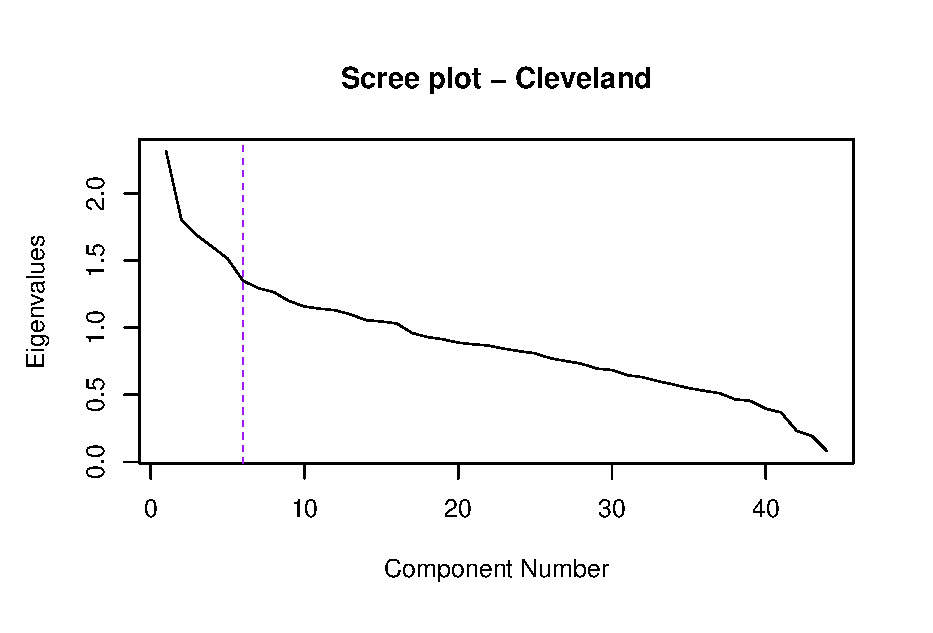
\includegraphics[width=15cm]{question3output/clescreeplot.eps} 
	\end{center}
	\caption{Screeplot for PCA of Cleveland}
	\label{q3-cle-screeplot}
\end{figure}


% From PCA we have the following importance of variables:

% \lstinputlisting[frame=single]{question3output/clepcaimportance.txt}

% Here we see that it is need for first 21 components in order to keep $80\%$ of the variance. 

\subsubsection{Hungary}

\subsubsection{Longbeach}

\subsubsection{Switzerland}

\subsection{Question 4}

\section{Summary}

\end{document}
